\documentclass[tikz,usenames,dvipsnames,border=10pt]{standalone}
% \usepackage[dvipsnames]{xcolor}
\usepackage{pgfplots}
\pgfplotsset{compat=1.16}
\usepgfplotslibrary{statistics}


\begin{document}

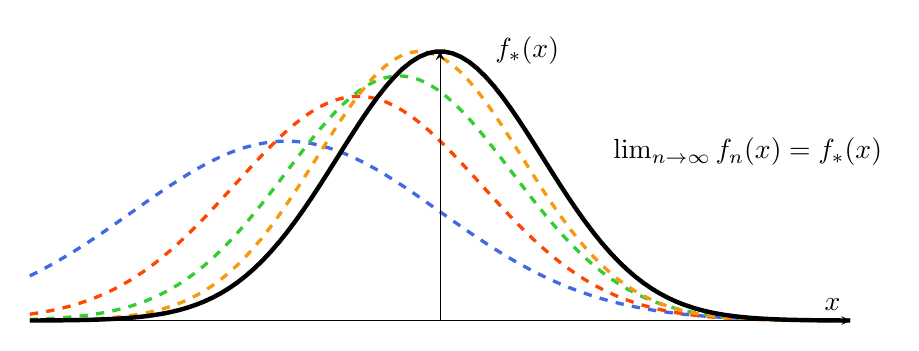
\begin{tikzpicture}
\begin{axis}[
  no markers, 
  domain=-4:4, 
  samples=100,
  ymin=0,
  axis lines*=left, 
  xlabel=\( x \),
  height=5cm, 
  width=12cm,
  xtick=\empty, 
  ytick=\empty,
  enlargelimits=false, 
  clip=false, 
  axis on top,
  grid = major,
  axis lines = middle
]


% Approaching distributions
\addplot [very thick,RoyalBlue, dashed] {1/(1.5*sqrt(2*pi))*exp(-((x+1.5)^2)/(2*1.5^2))};
\addplot [very thick,OrangeRed, dashed] {1/(1.2*sqrt(2*pi))*exp(-((x+0.8)^2)/(2*1.2^2))};
\addplot [very thick,LimeGreen, dashed] {1/(1.1*sqrt(2*pi))*exp(-((x+0.4)^2)/(2*1.1^2))};
\addplot [very thick,YellowOrange, dashed] {1/(1*sqrt(2*pi))*exp(-((x+0.2)^2)/(2*1^2))};

\node at (.85, .4) {$f_*(x)$};
\node at (3, .25) {$\lim_{n\to\infty} f_n(x) = f_*(x)$};

% Target distribution: mean = 0, std dev = 1
\addplot [ultra thick,black] {1/(1*sqrt(2*pi))*exp(-((x-0)^2)/(2*1^2))};

\end{axis}
\end{tikzpicture}

\end{document}
